\section{Results}
\label{sec:results}

\subsection{Natural onsets are rare and early}
\label{sec:data}

\begin{table}[t]
\centering
\small
\caption{Trajectories per prompt source. Event columns give the number of trajectories with the event (in parentheses: with onset $\ge$64 tokens, which can contribute positives at $H>64$). Unsafe onsets occur at 0, 64, 128, 256 and 448 tokens only.}
\label{tab:data}
\begin{tabular}{@{}lcccccc@{}}
\toprule
\textbf{Source} & \textbf{$n$} & \textbf{Test} & \textbf{Median len.} & \textbf{Ended \eos} & \textbf{Unsafe} & \textbf{Caution} \\
\midrule
\longwriter & 32 & 9 & 1559 & 21 & 2 (2) & 3 (3) \\
\toxicchat & 16 & 7 & 116 & 16 & 0 & 8 (0) \\
\beavertails & 16 & 4 & 127 & 16 & 2 (1) & 12 (0) \\
\aegis & 16 & 6 & 125 & 16 & 1 (1) & 12 (2) \\
\xstest & 16 & 2 & 242 & 16 & 0 & 7 (2) \\
\bottomrule
\end{tabular}
\end{table}


\Tabref{tab:data} summarizes the data.
Only 5 of 84 continuations contain a segment flagged unsafe, and every unsafe onset is at or before token 448.
Caution events are more frequent (42 trajectories), but most are refusals at token 0; only seven have a late onset (256, 384, 512, 768, 1152, 1152 and 1408 tokens).
Segment behaviors are dominated by explain (614 segments), narrate (234) and recommend (133); refuse (27) and warn (23) are rare.
Because 86\% of responses end with \eos and are censored, the number of known-status still-safe test prefixes falls quickly with horizon: 306, 282, 239, 175, 89 and 13 for $H = 64,\dots,2048$ on the unsafe event.
We therefore treat $H=2048$ as uninformative throughout.

\subsection{Unsafe-onset forecasting is unpowered}
\label{sec:unsafe}

\begin{table}[t]
\centering
\small
\caption{Unsafe-onset forecasting: AUROC on known-status still-safe test prefixes (mean $\pm$ sd over 3 seeds). Test positives per $H$ are 2/4/6/10/10/10 prefixes from only 2 event trajectories, so this event is unpowered; no observer differs significantly from \directao. Best per column in \textbf{bold}.}
\label{tab:unsafe}
\begin{tabular}{@{}lcccccc@{}}
\toprule
\textbf{Method} & $H{=}64$ & 128 & 256 & 512 & 1024 & 2048 \\
\midrule
Prevalence (KM) & 0.500 & 0.500 & 0.500 & 0.500 & 0.500 & 0.500 \\
Position & 0.697 & 0.729 & 0.704 & 0.751 & 0.685 & 0.900 \\
Linear probe & 0.658 & 0.710 & 0.771 & 0.841 & 0.820 & \textbf{0.933} \\
Text-only TF-IDF & \textbf{0.732} & \textbf{0.816} & \textbf{0.855} & \textbf{0.929} & \textbf{0.920} & \textbf{0.933} \\
\midrule
\directao & 0.530{\scriptsize$\pm$.04} & 0.527{\scriptsize$\pm$.01} & 0.710{\scriptsize$\pm$.01} & 0.805{\scriptsize$\pm$.02} & 0.825{\scriptsize$\pm$.01} & 0.878{\scriptsize$\pm$.02} \\
\hq & 0.502{\scriptsize$\pm$.04} & 0.494{\scriptsize$\pm$.03} & 0.668{\scriptsize$\pm$.02} & 0.758{\scriptsize$\pm$.04} & 0.777{\scriptsize$\pm$.04} & \textbf{0.933}{\scriptsize$\pm$.00} \\
\roll & 0.514{\scriptsize$\pm$.03} & 0.599{\scriptsize$\pm$.05} & 0.731{\scriptsize$\pm$.03} & 0.795{\scriptsize$\pm$.05} & 0.808{\scriptsize$\pm$.04} & 0.889{\scriptsize$\pm$.07} \\
\hier & 0.531{\scriptsize$\pm$.13} & 0.466{\scriptsize$\pm$.13} & 0.577{\scriptsize$\pm$.17} & 0.618{\scriptsize$\pm$.21} & 0.600{\scriptsize$\pm$.22} & 0.811{\scriptsize$\pm$.10} \\
\bottomrule
\end{tabular}
\end{table}


\Tabref{tab:unsafe} reports AUROC for the primary event.
The text-only TF-IDF baseline is best at every horizon (0.732--0.929 for $H \le 1024$), and the linear probe and \directao follow.
None of the memory-based observers improves on \directao, and every family-bootstrap 95\% CI for the difference includes zero.
Early-warning recall at a 5\% trajectory false-alarm rate is 0 for every method, since only one test trajectory has an onset at or after 128 tokens.
With 2 test event trajectories (onsets at 64 and 448 tokens), {\bf we draw no architectural conclusion from this event}.

\subsection{Caution-onset forecasting}
\label{sec:caution}

\begin{figure}[t]
\centering
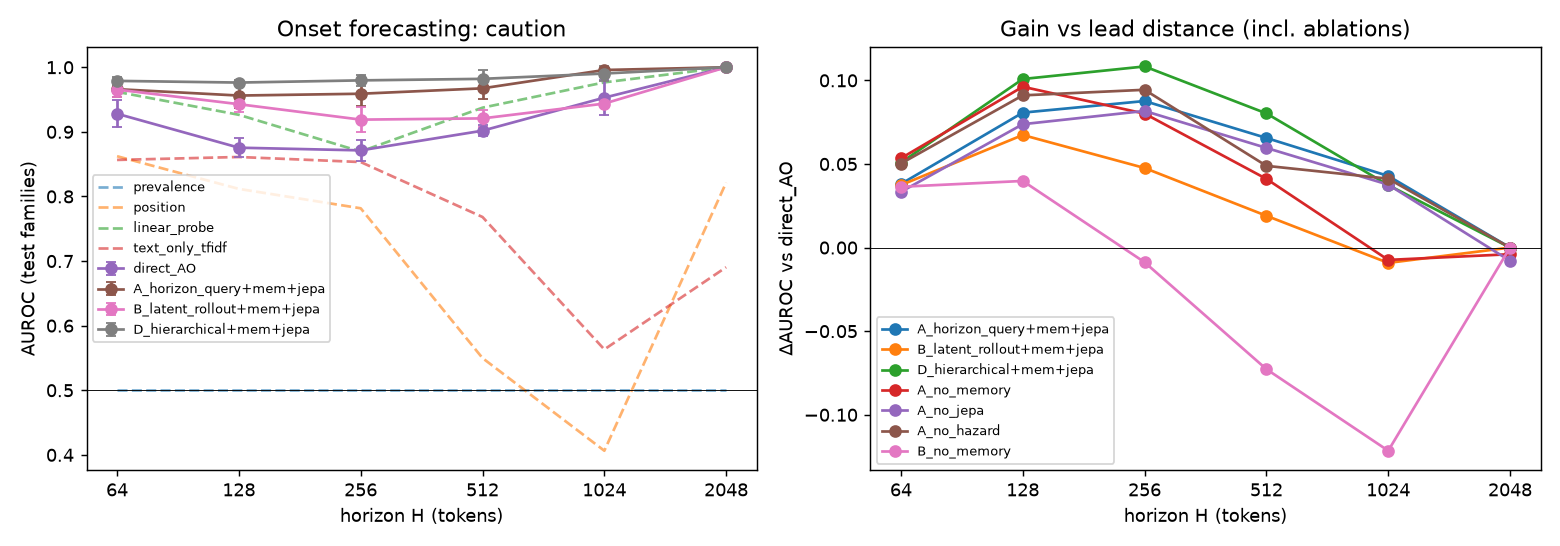
\includegraphics[width=0.95\linewidth]{figures/safety_auroc_vs_H_caution.png}
\caption{Caution-onset forecasting. \figleft AUROC vs.\ horizon for baselines (dashed) and observers (solid; error bars are seed sd). \figright $\Delta$AUROC vs.\ \directao, including ablations. The memory-based observers lead at every $H \le 1024$, but the gap peaks at $H = 128$--$256$ and shrinks by $H = 1024$; removing memory from \roll turns its gain negative at long horizons. All models reach 1.0 at $H = 2048$, where nearly all known-status prefixes are positive.}
\label{fig:caution}
\end{figure}

\begin{table}[t]
\centering
\caption{Caution-onset forecasting (first refuse/warn segment). \emph{Top:} AUROC on known-status still-safe test prefixes (mean $\pm$ sd over 3 seeds). \emph{Bottom:} $\Delta$AUROC vs.\ \directao with seed-averaged risk and 95\% family-cluster bootstrap CIs. $H{=}2048$ is omitted: only 31 known-status prefixes remain and nearly all are positive. Best per column in \textbf{bold}.}
\label{tab:caution}
\resizebox{\textwidth}{!}{%
\begin{tabular}{@{}lccccc@{}}
\toprule
\textbf{Method} & $H{=}64$ & 128 & 256 & 512 & 1024 \\
\midrule
Position & 0.862 & 0.812 & 0.782 & 0.550 & 0.406 \\
Text-only TF-IDF & 0.857 & 0.861 & 0.853 & 0.768 & 0.563 \\
Linear probe & 0.962 & 0.926 & 0.870 & 0.937 & 0.977 \\
\midrule
\directao & 0.928{\scriptsize$\pm$.02} & 0.875{\scriptsize$\pm$.01} & 0.871{\scriptsize$\pm$.02} & 0.902{\scriptsize$\pm$.01} & 0.953{\scriptsize$\pm$.03} \\
\hq (+memory, +JEPA, hazard) & 0.966{\scriptsize$\pm$.01} & 0.956{\scriptsize$\pm$.02} & 0.959{\scriptsize$\pm$.02} & 0.967{\scriptsize$\pm$.02} & \textbf{0.996}{\scriptsize$\pm$.00} \\
\roll (+memory, +JEPA, hazard) & 0.965{\scriptsize$\pm$.01} & 0.943{\scriptsize$\pm$.01} & 0.919{\scriptsize$\pm$.02} & 0.921{\scriptsize$\pm$.01} & 0.944{\scriptsize$\pm$.00} \\
\hier (+memory, +JEPA, hazard) & 0.979{\scriptsize$\pm$.01} & \textbf{0.976}{\scriptsize$\pm$.00} & \textbf{0.980}{\scriptsize$\pm$.01} & \textbf{0.982}{\scriptsize$\pm$.01} & 0.990{\scriptsize$\pm$.01} \\
\midrule
\hq $-$ memory & \textbf{0.981}{\scriptsize$\pm$.01} & 0.972{\scriptsize$\pm$.01} & 0.951{\scriptsize$\pm$.01} & 0.943{\scriptsize$\pm$.01} & 0.946{\scriptsize$\pm$.01} \\
\hq $-$ JEPA & 0.961{\scriptsize$\pm$.02} & 0.949{\scriptsize$\pm$.02} & 0.953{\scriptsize$\pm$.02} & 0.961{\scriptsize$\pm$.01} & 0.991{\scriptsize$\pm$.01} \\
\hq $-$ hazard head & 0.978{\scriptsize$\pm$.00} & 0.967{\scriptsize$\pm$.01} & 0.966{\scriptsize$\pm$.00} & 0.951{\scriptsize$\pm$.02} & 0.994{\scriptsize$\pm$.01} \\
\roll $-$ memory & 0.964{\scriptsize$\pm$.01} & 0.915{\scriptsize$\pm$.01} & 0.863{\scriptsize$\pm$.03} & 0.829{\scriptsize$\pm$.05} & 0.831{\scriptsize$\pm$.01} \\
\midrule
\multicolumn{6}{@{}l}{\emph{$\Delta$AUROC vs.\ \directao [95\% CI]}} \\
\hq & $+$0.03 [$-$.05, $+$.07] & $+$0.08 [$-$.05, $+$.15] & $+$0.09 [$-$.03, $+$.16] & $+$0.07 [$-$.02, $+$.13] & $+$0.03 [.00, $+$.09] \\
\roll & $+$0.03 [$-$.01, $+$.05] & $+$0.06 [$-$.01, $+$.10] & $+$0.05 [$-$.04, $+$.10] & $+$0.01 [$-$.06, $+$.06] & $-$0.01 [$-$.07, $+$.01] \\
\hier & $+$0.04 [$-$.02, $+$.07] & $+$0.10 [$-$.01, $+$.15] & $+$0.11 [.00, $+$.16] & $+$0.09 [.00, $+$.14], $p{=}.09$ & $+$0.03 [.00, $+$.09] \\
\roll $-$ memory & $+$0.02 & $+$0.03 & $-$0.02 & $-$0.08 [$-$.22, $+$.02] & $-$0.11 [$-$.20, .00], $p{=}.06$ \\
\bottomrule
\end{tabular}}
\end{table}


{\bf Do memory-based observers beat the direct readout?}
On the denser caution event, yes in sign, but not significantly (\tabref{tab:caution}, \figref{fig:caution}).
\hier reaches AUROC 0.976--0.990 at $H \le 1024$, compared with 0.871--0.953 for \directao, a difference of $+0.04$ to $+0.11$.
Its largest gains are at $H=256$ ($+0.11$, CI [0.00, 0.16]) and $H=512$ ($+0.09$, CI [0.00, 0.14], $p=0.09$).
\hq gains $+0.03$ to $+0.09$.
The gains are consistent across seeds, but every CI touches or includes zero, because only three test trajectories from two families have a late caution onset.
A plain linear probe on the latest activation is nearly as strong (0.870--0.977), which shows that most of the signal is already present in the current state.

{\bf Does the gain grow with lead distance?}
No.
The gap over \directao peaks at $H = 256$--$512$ and shrinks to $+0.03$ at $H=1024$ (\figref{fig:caution}, right).
Part of this shrinkage is a ceiling: \directao itself reaches 0.953 at $H=1024$.
\hier has the flattest curve of all models.

{\bf Which components matter?}
\emph{Memory} gives the clearest long-horizon benefit.
Removing it from \roll lowers AUROC from 0.921 to 0.829 at $H=512$ and from 0.944 to 0.831 at $H=1024$ ($\Delta$ vs.\ \directao $=-0.11$, $p=0.06$).
Removing it from \hq lowers AUROC at $H=1024$ from 0.996 to 0.946.
At short horizons memory does not help: \hq without memory is the best model at $H=64$ (0.981).
\emph{The JEPA auxiliary} changes AUROC by about 0.01 at every horizon.
\emph{The hazard head} gives no AUROC gain over independent per-$H$ classifiers (\hq $-$ hazard head is within 0.016 of \hq everywhere).
\emph{Latent rollout} does not reach further than direct query-based prediction: \roll is the weakest memory-based observer at $H \ge 256$.

{\bf Calibration.}
At $H \le 512$ all activation models have similar Brier scores (0.015--0.09, vs.\ 0.03--0.12 for prevalence).
At $H = 1024$, \directao scores 0.082 and \hq without the hazard head 0.065, while the hazard models score 0.08--0.11 and \roll without memory 0.16.
At $H=2048$ the hazard models with memory degrade to 0.24--0.30, compared with 0.02--0.03 for independent per-$H$ classifiers.
They under-predict because \eqref{eq:hazard} must extrapolate the hazard over late bins that are rarely observed in training.

{\bf Early warning.}
Only 3 test trajectories have a caution onset at or after 128 tokens.
Recall at a 5\% trajectory false-alarm rate is 0/3 for all observers except \hq without JEPA (1/3), and 2/3 for TF-IDF; these counts are too small to compare methods.

\subsection{Pooled AUROC largely reflects prompt type}
\label{sec:per_source}

{\bf Is the caution gain a timing forecast?}
Mostly not.
At $H \ge 512$, all positive test prefixes for the caution event come from \aegis and \xstest prompts, while \longwriter prefixes, the majority, are all negative.
A model that separates harmful-looking prompts from long-form tasks therefore scores high without forecasting timing.
Within a single source the evidence is thin (\tabref{tab:per_source} in \appref{app:per_source}).
On the 9 \xstest prefixes at $H=512$, AUROC is 1.00 for \hier, 0.50 for \roll, 0.38 for \directao and 0.00 for \hq.
On the unsafe event, within \aegis (14 prefixes, 8 positive), \hier and \hq without JEPA reach 0.94 vs.\ 0.85 for \directao, while within \longwriter (2 positives) every model is at or below chance (0.11--0.55).
We therefore read pooled differences as ``which observer better encodes prompt-type risk'' rather than as evidence of long-range timing forecasts.

\subsection{Long-form content forecasting}
\label{sec:content}

\begin{figure}[t]
\centering
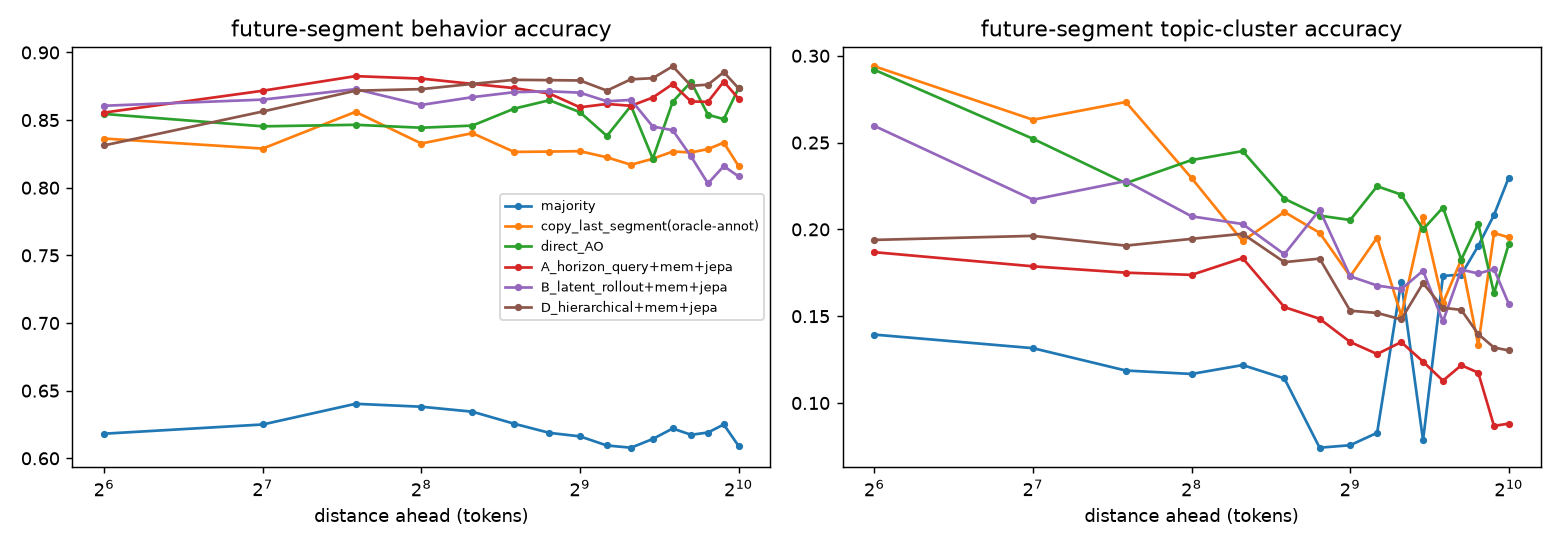
\includegraphics[width=0.95\linewidth]{figures/content_vs_distance_unsafe.png}
\caption{Content forecasting vs.\ distance ahead. \figleft Future-segment behavior accuracy: all observers stay at 0.83--0.89 up to 1024 tokens ahead, above the majority baseline (about 0.62) and slightly above copy-last-segment, which uses annotator labels. \figright Topic-cluster accuracy: \directao and copy-last are strongest; the query-based observers \hq and \hier are weakest and decline with distance.}
\label{fig:content}
\end{figure}

\begin{table}[t]
\centering
\caption{Long-form content forecasting on all test cutoffs. Behavior accuracy (7-way) and topic-cluster accuracy (16-way) at distance $k$ segments (64 tokens each), and remaining-response summary retrieval among 330 test cutoffs. Copy-last uses the annotator's label of the last observed segment. Seed sd is $\le$0.02 for most cells (0.06 for \roll at $k{=}16$). Best per column in \textbf{bold}.}
\label{tab:content}
\resizebox{\textwidth}{!}{%
\begin{tabular}{@{}lcccccccccc@{}}
\toprule
& \multicolumn{4}{c}{\textbf{Behavior acc.}} & \multicolumn{4}{c}{\textbf{Topic acc.}} & \multicolumn{2}{c}{\textbf{Summary}} \\
\cmidrule(lr){2-5} \cmidrule(lr){6-9} \cmidrule(lr){10-11}
\textbf{Method} & $k{=}1$ & 4 & 8 & 16 & $k{=}1$ & 4 & 8 & 16 & MRR & Top-10 \\
\midrule
Majority per distance & 0.618 & 0.638 & 0.616 & 0.609 & 0.139 & 0.117 & 0.076 & \textbf{0.230} & 0.019 & 0.030 \\
Copy last segment & 0.836 & 0.833 & 0.827 & 0.816 & \textbf{0.294} & 0.230 & 0.173 & 0.195 & 0.019 & 0.030 \\
\midrule
\directao & 0.855 & 0.844 & 0.856 & \textbf{0.874} & 0.292 & \textbf{0.240} & \textbf{0.205} & 0.192 & 0.087 & 0.200 \\
\hq & 0.856 & \textbf{0.881} & 0.859 & 0.866 & 0.187 & 0.174 & 0.135 & 0.088 & 0.095 & 0.235 \\
\roll & 0.861 & 0.861 & 0.870 & 0.808 & 0.260 & 0.208 & 0.173 & 0.157 & 0.074 & 0.160 \\
\hier & 0.831 & 0.873 & \textbf{0.879} & \textbf{0.874} & 0.194 & 0.195 & 0.153 & 0.130 & 0.099 & 0.239 \\
\midrule
\hq $-$ memory & 0.829 & 0.869 & 0.872 & 0.862 & 0.238 & 0.202 & 0.202 & 0.176 & \textbf{0.101} & 0.249 \\
\hq $-$ JEPA & \textbf{0.862} & 0.873 & 0.859 & 0.870 & 0.195 & 0.180 & 0.135 & 0.100 & 0.094 & 0.239 \\
\hq $-$ hazard head & 0.860 & 0.879 & 0.870 & 0.870 & 0.178 & 0.157 & 0.139 & 0.092 & 0.098 & \textbf{0.257} \\
\roll $-$ memory & 0.858 & 0.850 & 0.841 & 0.785 & 0.256 & 0.223 & 0.200 & 0.180 & 0.076 & 0.179 \\
\bottomrule
\end{tabular}}
\end{table}


{\bf Can observers forecast what a long response will do?}
Yes, for behavior and summaries (\tabref{tab:content}, \figref{fig:content}).
All activation observers forecast future-segment behavior at 0.83--0.88 accuracy up to 1024 tokens ahead, far above the majority baseline (0.61--0.64) and slightly above copy-last (0.82--0.84).
Summary retrieval reaches MRR 0.074--0.101, compared with 0.019 for the no-activation baselines, a 4--5$\times$ improvement.
\hq and \hier beat \directao on summary retrieval (MRR 0.095 and 0.099 vs.\ 0.087; top-10 0.235 and 0.239 vs.\ 0.200) and on behavior at 256--512 tokens ahead (0.873--0.881 vs.\ 0.844--0.856).
\directao is best on topic-cluster accuracy at $k \ge 4$, where \hq falls to 0.088 at $k=16$.
Here memory is not needed: \hq without memory has the best MRR (0.101).

{\bf Do observers actually read activations?}
Yes.
Zeroing activations at test time drops behavior accuracy at $k=4$ to the majority value (0.638) or below (0.06 for \directao), and summary MRR to chance (0.019).
Shuffling activations across trajectories gives behavior accuracy 0.46--0.52 and MRR 0.024--0.031.
One caveat: for memory models with zeroed inputs, the padding mask still reveals the cutoff position, which explains above-chance zero-control safety AUROC for some memory models.

\subsection{Cost}
\label{sec:cost}

\begin{table}[t]
\centering
\small
\caption{Cost on one RTX A6000. About 4.2M parameters of each budget are the shared $16384\to256$ input projection.}
\label{tab:cost}
\begin{tabular}{@{}lccc@{}}
\toprule
\textbf{Model} & \textbf{Params} & \textbf{Train time / seed} & \textbf{Latency / 16-token update} \\
\midrule
\directao & 6.00M & 1 s & 0.9 ms \\
\hq & 5.97M & 3 s & 2.3 ms \\
\roll & 5.84M & 4 s & 3.8 ms \\
\hier & 6.04M & 3 s & 2.5 ms \\
\bottomrule
\end{tabular}
\end{table}


All observers are cheap (\tabref{tab:cost}).
Memory-based observers cost 2.3--3.8\,ms per 16-token update, compared with 0.9\,ms for \directao, and train in 3--4\,s per seed on our data.
